\documentclass{article}

% if you need to pass options to natbib, use, e.g.:
% \PassOptionsToPackage{numbers, compress}{natbib}
% before loading nips_2017
%
% to avoid loading the natbib package, add option nonatbib:
% \usepackage[nonatbib]{nips_2017}

\usepackage[final]{ner}

% to compile a camera-ready version, add the [final] option, e.g.:
% \usepackage[final]{nips_2017}

\usepackage[utf8]{inputenc} % allow utf-8 input
\usepackage[T1]{fontenc}    % use 8-bit T1 fonts
\usepackage{hyperref}       % hyperlinks
\usepackage{url}            % simple URL typesetting
\usepackage{booktabs}       % professional-quality tables
\usepackage{amsfonts}       % blackboard math symbols
\usepackage{nicefrac}       % compact symbols for 1/2, etc.
\usepackage{microtype}      % microtypography
\usepackage{subcaption}
\usepackage{amsmath}

\usepackage[pdftex]{graphicx}
\usepackage{fancyhdr}
\usepackage[subpreambles=true]{standalone} 
\usepackage{tikz}

\usepackage{array}
\usepackage{amsfonts}
\usepackage{mathbbol}
\usepackage[ruled]{algorithm}
\usepackage{algpseudocode}

%% abbreviations
\newcommand{\ie}{\textit{i.e.}}
\newcommand{\st}{\textit{s.t.}}
\newcommand{\eg}{\textit{e.g.}}
\newcommand{\etc}{\textit{etc}}
\newcommand{\etal}{\textit{et~al.}}
\newcommand{\tuple}[1]{\ensuremath{( #1 )}\xspace}


\title{\nrc: a decentralized platform for Human-Robot Communication}

% The \author macro works with any number of authors. There are two
% commands used to separate the names and addresses of multiple
% authors: \And and \AND.
%
% Using \And between authors leaves it to LaTeX to determine where to
% break the lines. Using \AND forces a line break at that point. So,
% if LaTeX puts 3 of 4 authors names on the first line, and the last
% on the second line, try using \AND instead of \And before the third
% author name.

% An example of author info
%Chen Min\thanks{Use footnote for providing further
%information about author (webpage, alternative
%address)---\emph{not} for acknowledging funding agencies.} \\
%Department of Computer Science\\
%NUS, Singapore\\
%\texttt{chenmin@comp.nus.edu.sg} \\

\author{
  Chen Min, PhD\thanks{Expected to graduate in Aug 2018}\\
  NEO Robotics
  \\
  NUS, Singapore\\
  \texttt{chenmin@comp.nus.edu.sg} \\
  \And
  Xie Shudong, PhD\thanks{Expected to graduate in Dec 2017}\\
  NEO Robotics
  \thanks{NEO Robotics is the name of our team.
      The objective of our team is to use blockchain technology
      to improve robots' capabilities and safety when working 
      with humans.}
  \\
  Singapore\\
  \texttt{purplebamboot@gmail.com} \\
  \And
  Chen Liyuan, Msc\\
  NEO Robotics\\
  Singapore\\
  \texttt{colacly@gmail.com} \\
  %% examples of more authors
  %% \And
  %% Coauthor \\
  %% Affiliation \\
  %% Address \\
  %% \texttt{email} \\
  %% \AND
  %% Coauthor \\
  %% Affiliation \\
  %% Address \\
  %% \texttt{email} \\
  %% \And
  %% Coauthor \\
  %% Affiliation \\
  %% Address \\
  %% \texttt{email} \\
  %% \And
  %% Coauthor \\
  %% Affiliation \\
  %% Address \\
  %% \texttt{email} \\
}

\begin{document}
% \nipsfinalcopy is no longer used

\maketitle

\begin{abstract}
	
More and more robots are coming into human's daily life,
\eg, autonomous driving car and household robot.
Unlike traditional robots in the factory, robots that share the
same workspace with humans have to (i) gather information on humans'
physical state and mental state;
and (ii) take actions to achieve their own objectives.
Currently, most robots rely purely on onboard sensors to gather 
information, such as lidar and camera.
However, those sensors might fail due to weather or lighting
conditions, which might result in fatal accidents.
% topic
This paper introduces NRC, 
a decentralized platform built on NEO blockchain
for trust-free human-robot communication.
With \nrc, the human and the robot are able to broadcast their
information via blockchain, and receive the 
information of other agents for decision making.
% the adavantage of NER, and the impact
% 1. compared with onboard sensors
Compared with the onboard sensors, NRC can provides additional 
information for the robot, which can not be achieved by onboard
sensors.
For example, with \nrc, the robot will be able to know the 
position of the
human when they are separated by an obstacle in the middle, 
% 2. compared with the traditional communication device
Compared to the traditional communication devices, the blockchain based
NRC provides serveral adavantages:
(i) it reduces the cost of trust, \ie, the human and the robot can trust
the information they received is correct. This is handled automatically
by the blockchain technology without any extra effort.
(ii) the NRC token gives incentive for the human to share
their information to the robots, \ie, the human gets paid instantly
when his/her information is used by a robot.
As a proof of concept, we test NRC in the scenario of autonomous driving,
where we demonstrate the adavantages that NRC provides.
Note that NRC is general and not limit to autonomous driving. 
It can
be potentially applied on any robots that share their workspace
with humans, \eg, service robots in restaurants or hospitals.
 
\end{abstract}


\section{Introduction}

% Motivation
In the past decades, dramatic prograss has been made in the field
of robotics.
Robots are moving from factories, where robots have their own workspace,
into people's daily life, where robots share their workspace with humans (\figref{fig:robots}).
% Examples
There is an urgent need for developing robotic systems that can work closely with
human without hurting human or disturbing human's working flow.

\begin{figure}[t!]
    \centering
    \begin{tabular}{rr}
        \begin{subfigure}{0.99\linewidth}
            \centering
            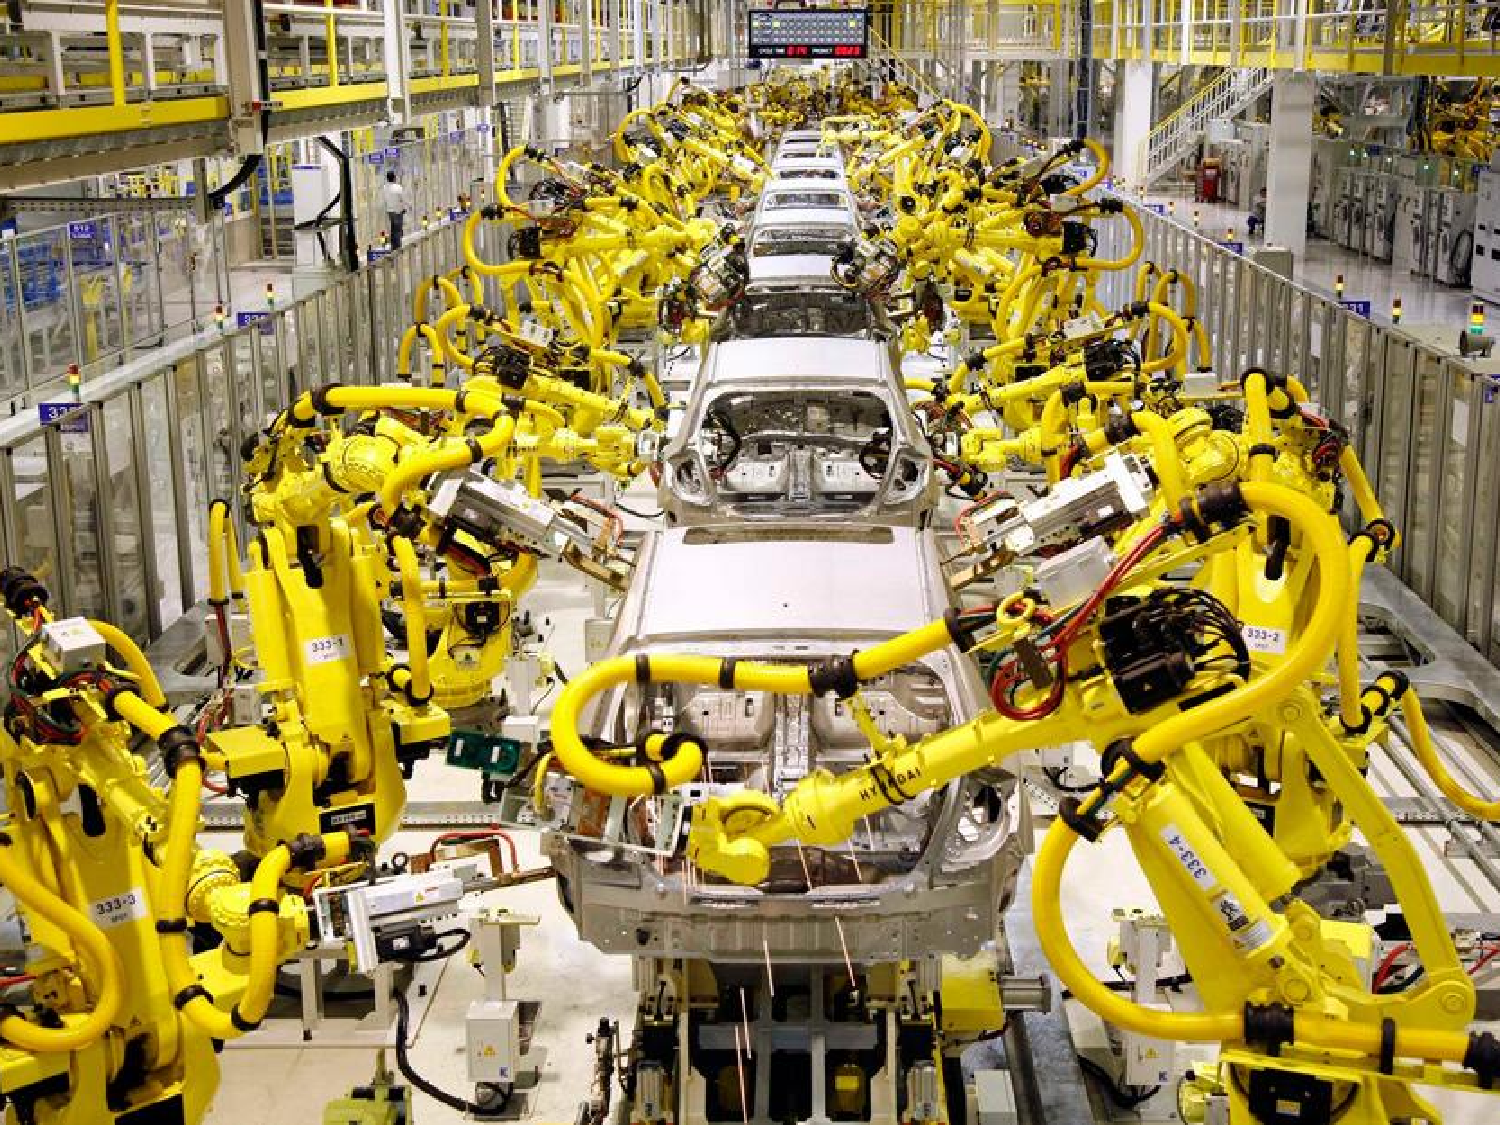
\includegraphics[width=.5\linewidth]{figs/industrial_robot.pdf} \\
        \end{subfigure}
        \\
        \\
        \\
        \\
        %\begin{tabular}{ccc}
        \begin{subfigure}{1.0\linewidth}
            \centering
            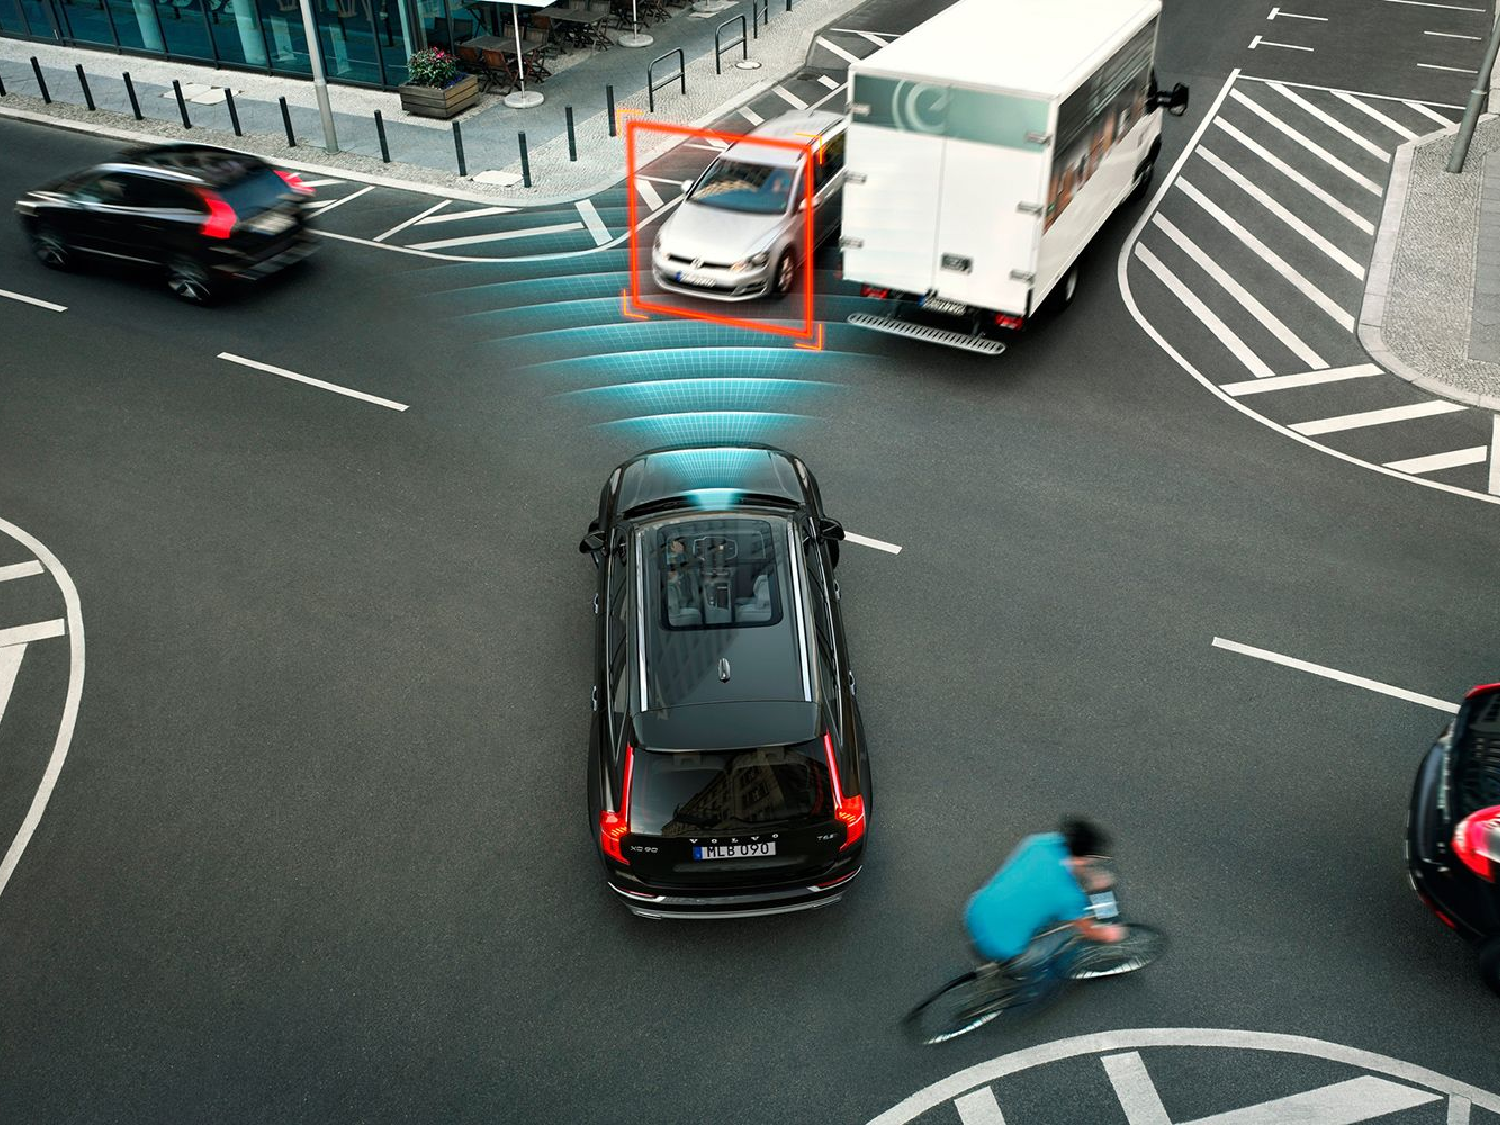
\includegraphics[width=.3\linewidth]{figs/autonomous_car.pdf} 
            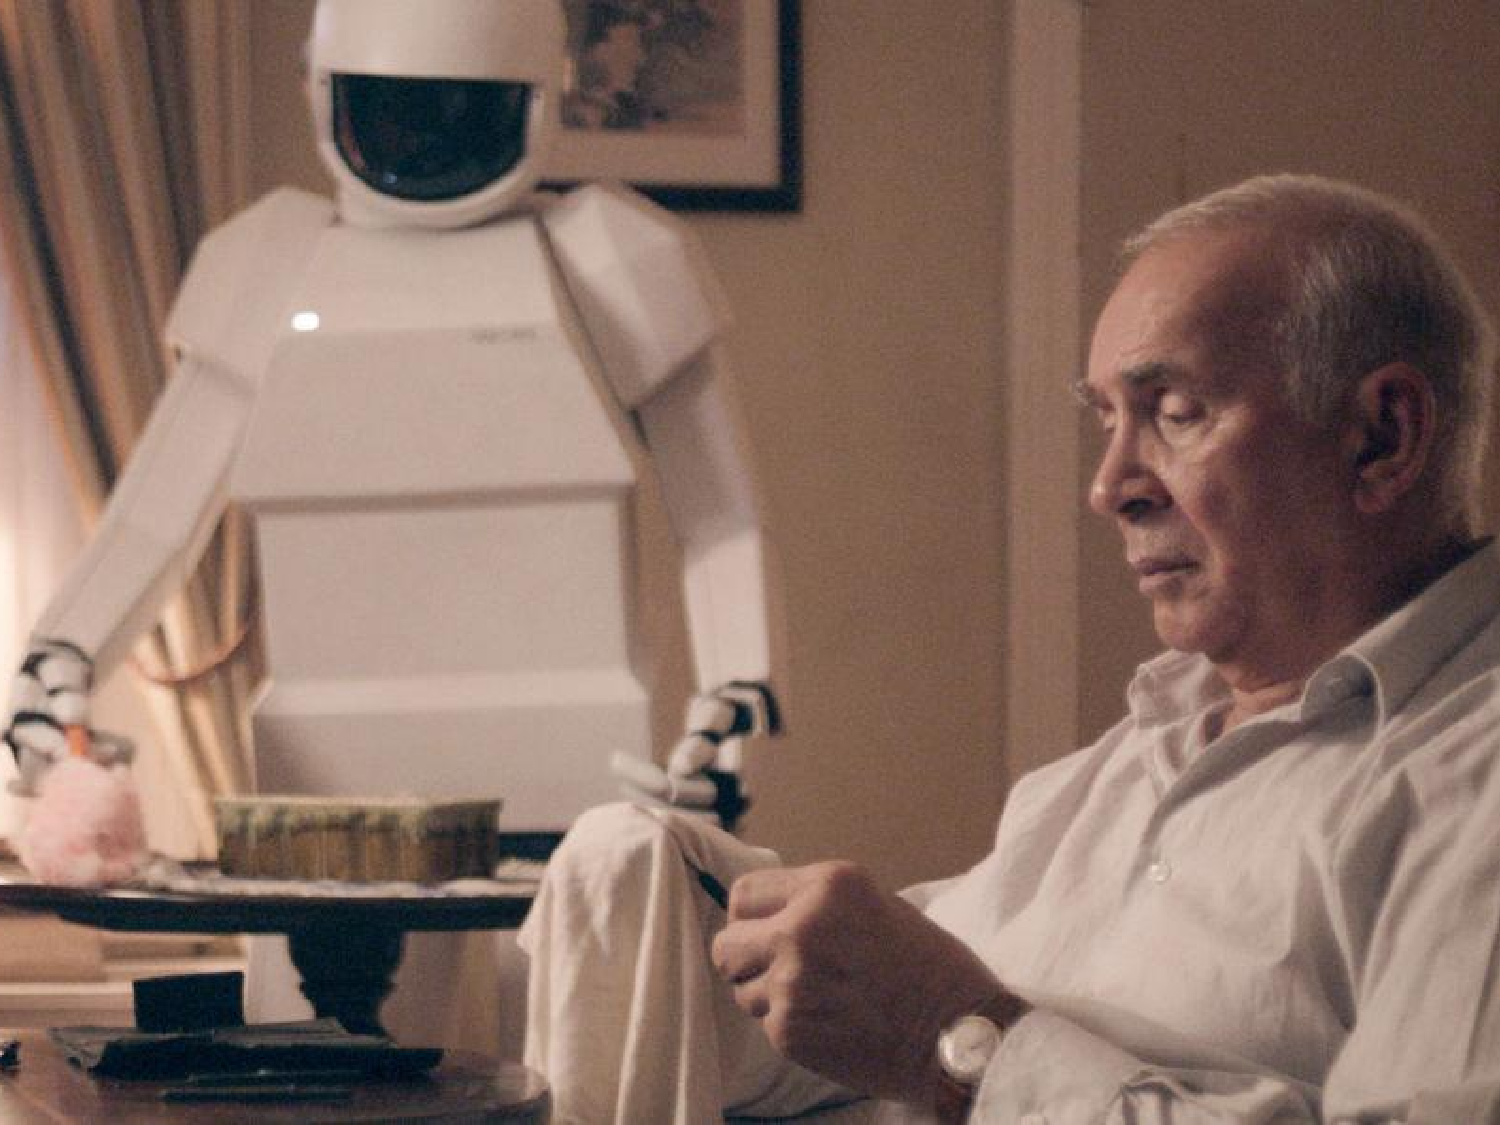
\includegraphics[width=.3\linewidth]{figs/homecare_robot.pdf} 
            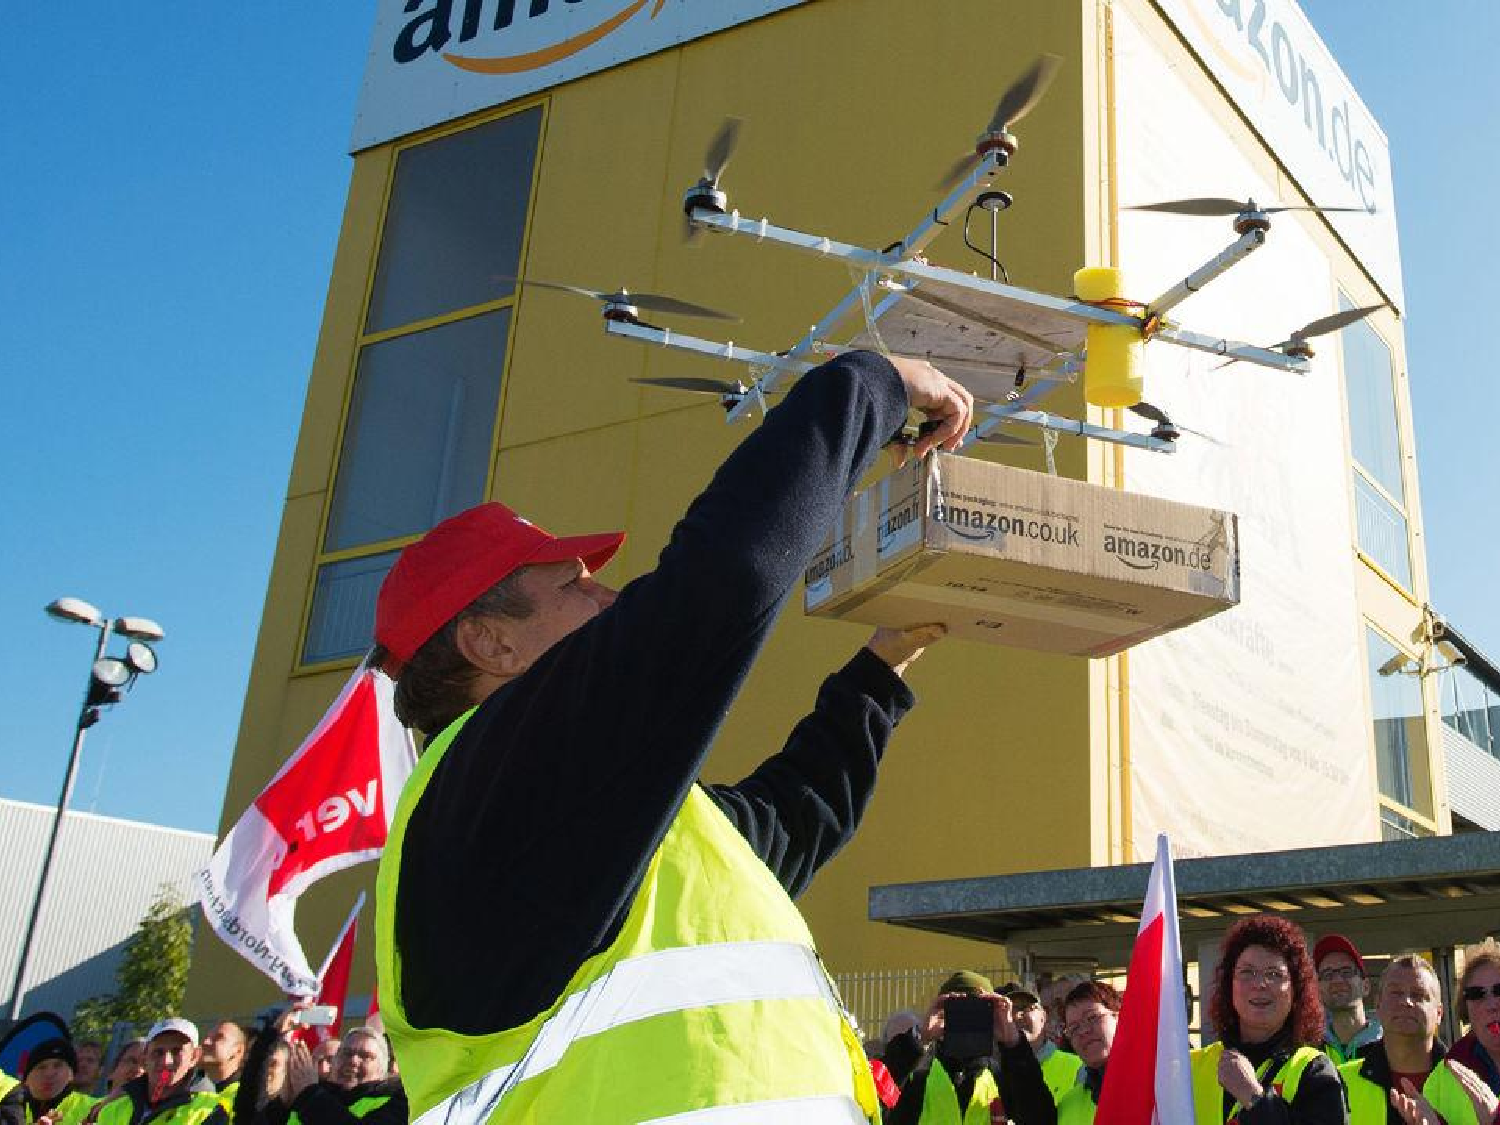
\includegraphics[width=.3\linewidth]{figs/drone_delivery.pdf} 
        \end{subfigure}
    \end{tabular}
    \caption{Top: Robots have their own workspace.
        Bottom: Robots share their workspace with humans.}
    \label{fig:robots}
\end{figure}

% challenges in robot collaborating with humans
Unlike industrial robots,
robot that working closely with human has to 
reason over human's 
physical state and mental state;
and plan its own actions accordingly.

\begin{figure}[!h]
    \centering
    \begin{subfigure}{1.0\linewidth}
        \centering
        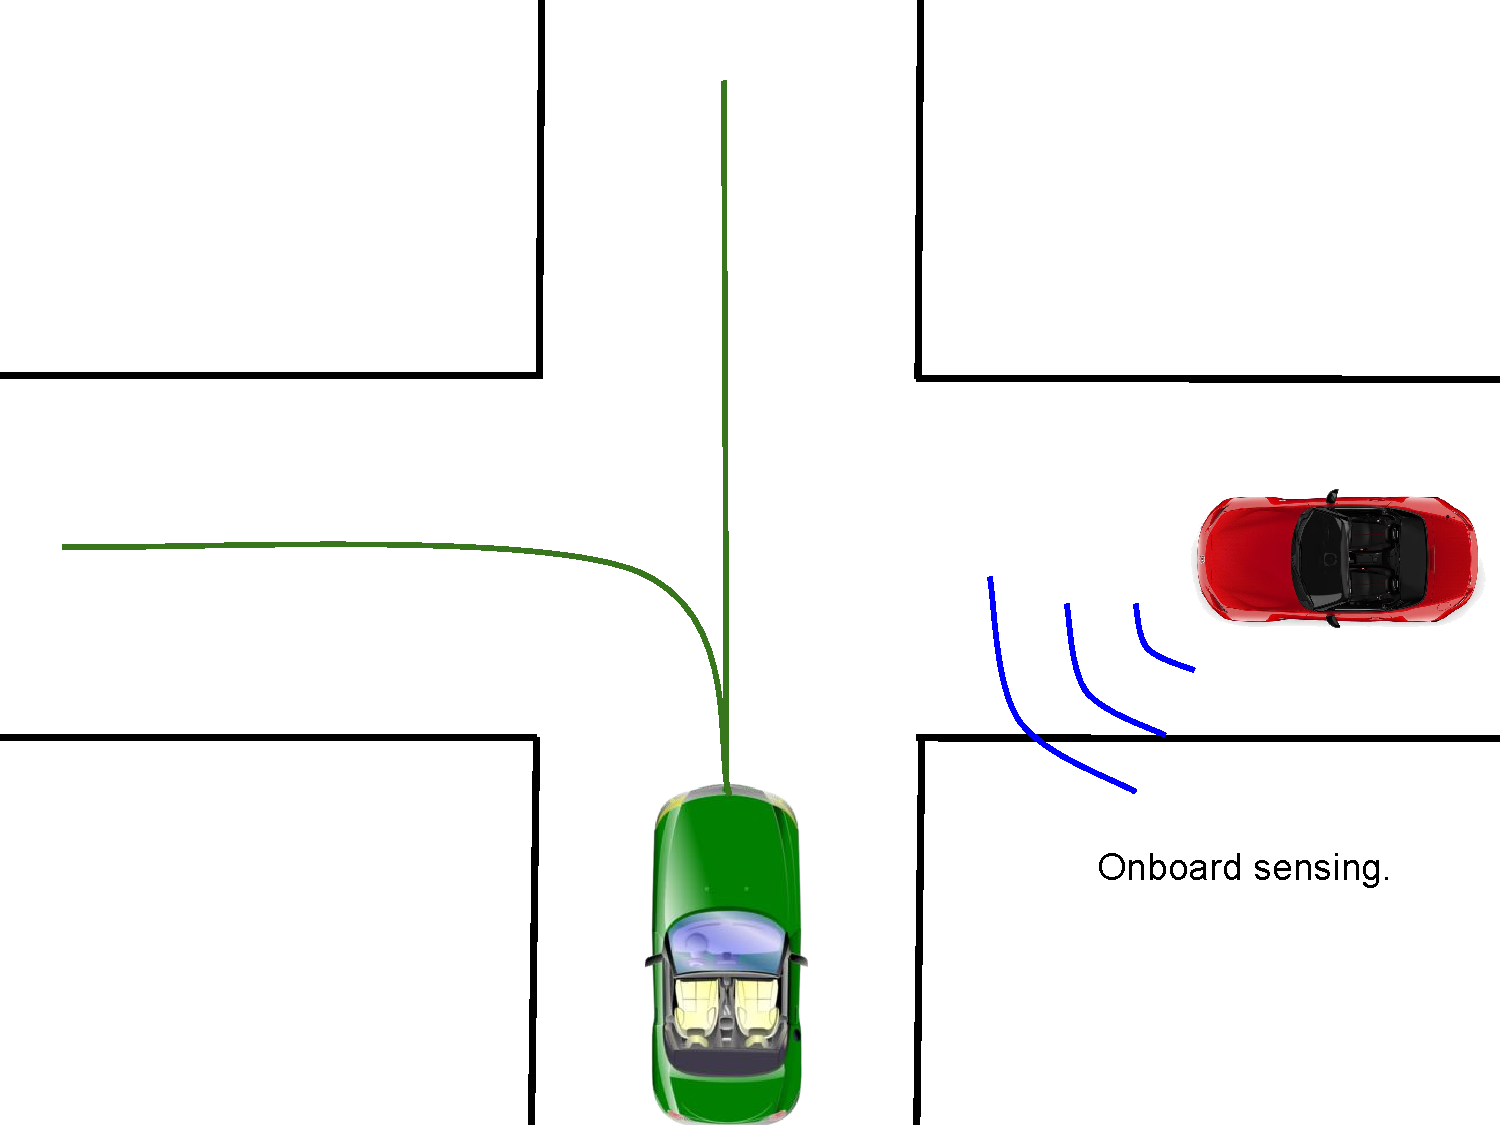
\includegraphics[width=0.4\linewidth]{intersection_nav.pdf}
        \hspace{1.5cm}
        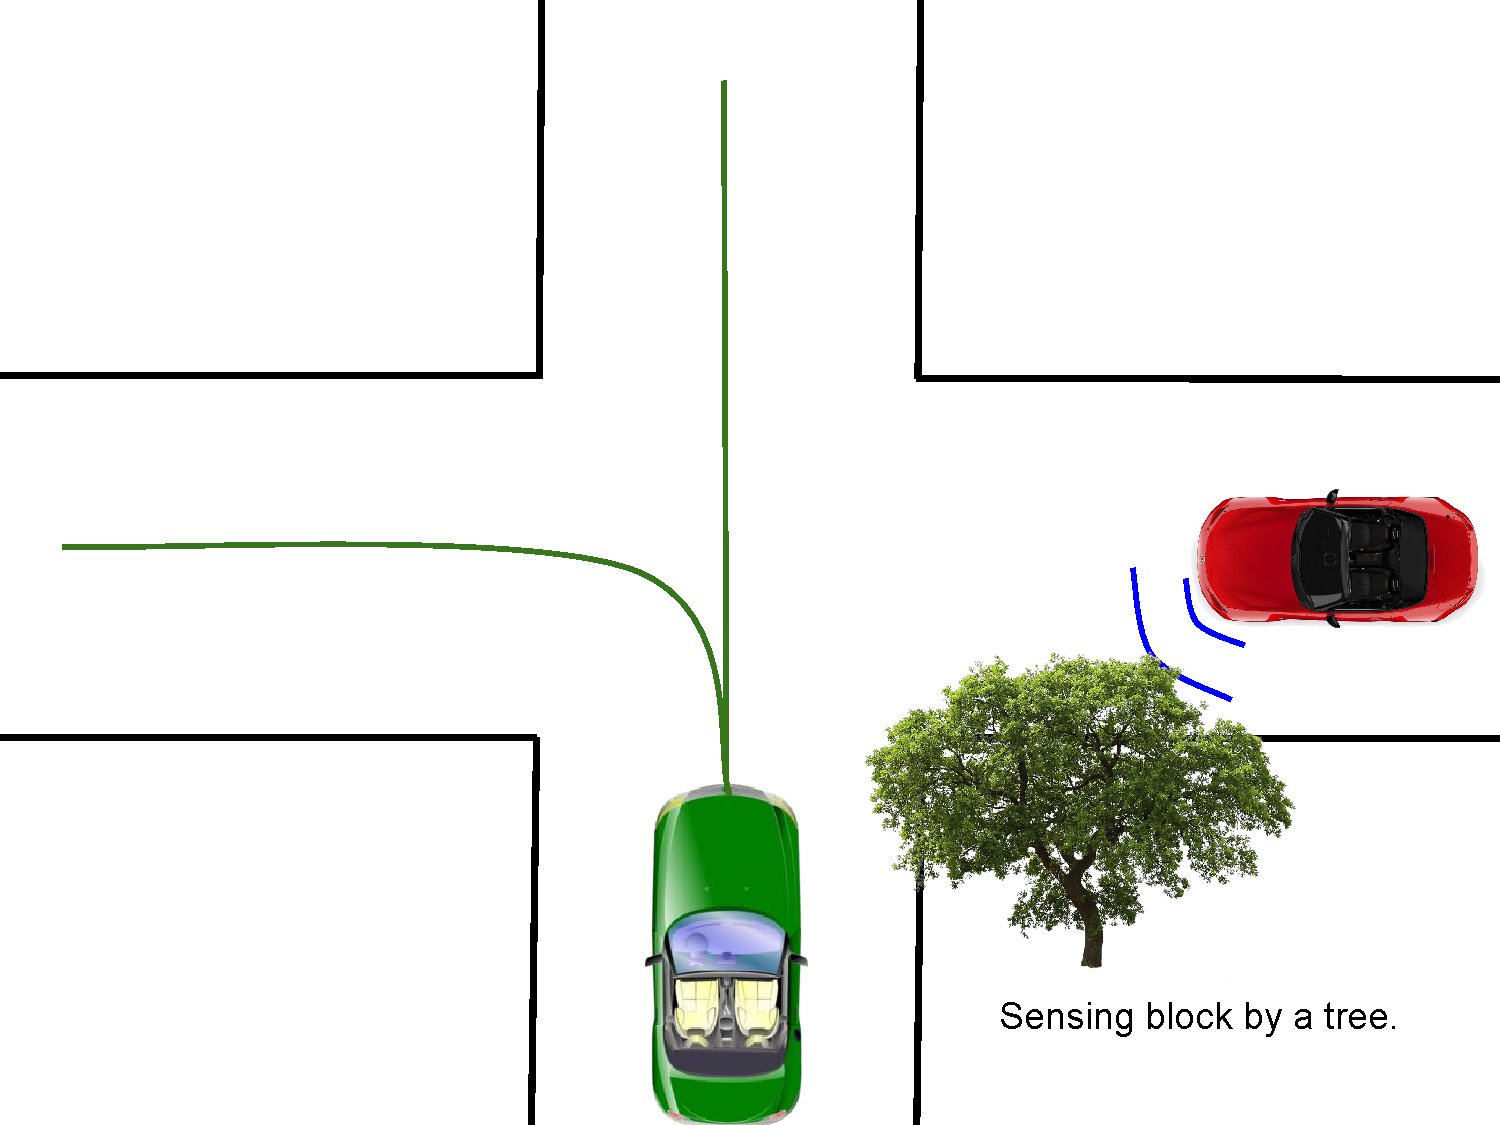
\includegraphics[width=0.4\linewidth]{intersection_nav_block.pdf}
    \end{subfigure}
    \caption{Left column:
        Autonomous car (red) navigating through an unsignalized 
        intersection, with another human driven car (green) around. 
        Right column:
        The onboard sensors might fail due to unexpected obstacles,
        \eg, trees around the road.
    }
    \label{fig:intersection_nav}
\end{figure}


% take an example to explain what is human's mental state, and why it is difficult
Consider an autonomous driving example in~\figref{fig:intersection_nav} (left column).
The autonomous car tries to navigate through an unsignalized intersection
while interacting with another human driver on road. 
Although it is a trival task for human drivers, it
turns out to be extremely difficult for a robot car to perform 
well in such scenario. 
In order to be safe and efficient, 
the robot car needs to 
know the positions of nearby human driven cars and the paths that 
human drivers are following.


% Current robots rely on onboard sensors
Nowadays, most robots rely purely on onboard sensors,
\eg, lidar and camera \etc,
to gather information from the environment. 
Onboard sensors provides only limited information for the
robot due to the following reasons.
\begin{itemize}
    \item Onboard sensors lack the ability to read humans' mental 
        state, \eg, the sensors will not be able to tell 
        which direction the huma driver is going
        (\figref{fig:intersection_nav}, left column).
    \item Onboard sensors can fail due to unexpected weather
        conditions or obstacles, \eg, the sensors is blocked
        by a tree in the autonomous driving task
        (\figref{fig:intersection_nav}, right column).
\end{itemize}


% Introduce NRC
In this paper, we introduce \nrc, a dApp based 
on NEO blockchain that enables trust-free human-robot 
communication.


% Differentiate NRC from traditional communication devices


% Preliminary results on testing NRC on a robot platform
We tested \nrc on the autonomous driving task as a proof of
concept.
(TODO: Preliminary results)


% Impact of NRC
We believe that robots will become more and more popular in
people's daily life, and \nrc provides a general solution
for human-robot information sharing.
Note that, although we demonstrated \nrc on the autonomous
driving task, \nrc is much more general and it can
be potentially applied on any robots that share their workspace
with humans, \eg, service robots in restaurants or hospitals.


\section{Background}
\label{sec:background}

\subsection{Onboard sensors for robot information gathering}
\label{subsec:onboard-sensors}

\subsection{Traditional communication devices}
\label{subsec:tranditional-communication}

\subsection{The NEO blockchain}
\label{subsec:neo-blockchain}

This part may introduce the current problems faced by robotics in information sharing.

\section{NRC for human-robot communication}
\label{sec:nrc}

\subsection{Model}
\label{subsec:model}

\subsection{Prototype dAPP}
\label{subsec:prototype}


\section{NRC token}

\subsection{Incentives for humans to share their information 
    with robots}



\subsection{Reward scheme}
What is the reward people can gain by sharing the information.


\section{Proof of concept}
\label{sec:proof-concept}

We can demostrate some interesting examples in this part.

\subsubsection{Robot seeing through the wall}

%\subsubsection{Case Study 2: Avoid the Tesla fatal crash while using autopilot mode}

\section{Roadmap}
\label{sec:roadmap}

We are going to achieve what goals by what time.


%\section*{References}

%References follow the acknowledgments. Use unnumbered first-level
%heading for the references. Any choice of citation style is acceptable
%as long as you are consistent. It is permissible to reduce the font
%size to \verb+small+ (9 point) when listing the references. {\bf
  %Remember that you can go over 8 pages as long as the subsequent ones contain
  %\emph{only} cited references.}

%\medskip

\small

\bibliographystyle{named}
\bibliography{ner}

\end{document}
